%\documentclass[handout]{beamer} 
\documentclass[t,12pt,numbers,fleqn]{beamer}
%\documentclass[ignorenonframetext]{beamer}

\newif\ifquestions
%\questionstrue
\questionsfalse

\usepackage{pgfpages} 
\usepackage{hyperref}
\hypersetup{colorlinks=true,
    linkcolor=blue,
    citecolor=blue,
    filecolor=blue,
    urlcolor=blue,
    unicode=false}
\urlstyle{same}

\usepackage{multicol}
\usepackage{booktabs}
\usepackage{bibentry}
\usepackage[round, authoryear]{natbib}
\bibliographystyle{plainnat}

\usepackage{tikz}
\usetikzlibrary{mindmap}
%tikstyle commands
% Define block styles
\tikzstyle{context} = [rectangle, rounded corners, text width=2.5cm, minimum
size=2.5cm,text centered, draw=black, fill=white!30]
\tikzstyle{strategy} = [trapezium, trapezium left angle=70, trapezium right
angle=110, text width=3cm, minimum height=1cm, text centered, draw=black,
fill=white!30]
\tikzstyle{subclaim} = [rectangle, text width=3cm, minimum height=1cm, text
centered, draw=black, fill=white!30]
\tikzstyle{goal} = [rectangle, text width=5cm, minimum height=1cm, text
centered, draw=black, fill=white!30]
\tikzstyle{assumption} = [ellipse, text width=3cm, minimum height=1cm, text
centered, draw=black, fill=white!30]
\tikzstyle{evidence} = [circle, text width=2cm, minimum size=2cm, text
centered,draw=black, fill=white!30]
\tikzstyle{arrow} = [thick,->,>=stealth]

\newcommand{\famname}{MIA}
\newcommand{\progname}{MISEG}

%\usetheme{Iimenau}

\useoutertheme{split} %so the footline can be seen, without needing pgfpages

%\pgfpagesuselayout{resize to}[letterpaper,border shrink=5mm,landscape]  %if this is uncommented, the hyperref links do not work

\mode<presentation>{}

%% Requires:
%% 
%% \usepackage{latexsym}
%% \usepackage{amssymb}
%% \usepackage{stmaryrd}

%\renewcommand{\labelenumi}{(\theenumi)}

\newcommand{\be}{\begin{enumerate}}
\newcommand{\ee}{\end{enumerate}}
\newcommand{\bi}{\begin{itemize}}
\newcommand{\ei}{\end{itemize}}
\newcommand{\bc}{\begin{center}}
\newcommand{\ec}{\end{center}}
\newcommand{\bsp}{\begin{sloppypar}}
\newcommand{\esp}{\end{sloppypar}}

\newcommand{\sglsp}{\ }
\newcommand{\dblsp}{\ \ }

\newcommand{\iclicker}{i\texttt{>}clicker}

\newcommand{\sA}{\mbox{$\cal A$}}
\newcommand{\sB}{\mbox{$\cal B$}}
\newcommand{\sC}{\mbox{$\cal C$}}
\newcommand{\sD}{\mbox{$\cal D$}}
\newcommand{\sE}{\mbox{$\cal E$}}
\newcommand{\sF}{\mbox{$\cal F$}}
\newcommand{\sG}{\mbox{$\cal G$}}
\newcommand{\sH}{\mbox{$\cal H$}}
\newcommand{\sI}{\mbox{$\cal I$}}
\newcommand{\sJ}{\mbox{$\cal J$}}
\newcommand{\sK}{\mbox{$\cal K$}}
\newcommand{\sL}{\mbox{$\cal L$}}
\newcommand{\sM}{\mbox{$\cal M$}}
\newcommand{\sN}{\mbox{$\cal N$}}
\newcommand{\sO}{\mbox{$\cal O$}}
\newcommand{\sP}{\mbox{$\cal P$}}
\newcommand{\sQ}{\mbox{$\cal Q$}}
\newcommand{\sR}{\mbox{$\cal R$}}
\newcommand{\sS}{\mbox{$\cal S$}}
\newcommand{\sT}{\mbox{$\cal T$}}
\newcommand{\sU}{\mbox{$\cal U$}}
\newcommand{\sV}{\mbox{$\cal V$}}
\newcommand{\sW}{\mbox{$\cal W$}}
\newcommand{\sX}{\mbox{$\cal X$}}
\newcommand{\sY}{\mbox{$\cal Y$}}
\newcommand{\sZ}{\mbox{$\cal Z$}}

\renewcommand{\phi}{\varphi}
\newcommand{\seq}[1]{{\langle #1 \rangle}}
\newcommand{\set}[1]{{\{ #1 \}}}
\newcommand{\tuple}[1]{{( #1 )}}
\newcommand{\mlist}[1]{{[ #1 ]}}
\newcommand{\sembrack}[1]{\llbracket#1\rrbracket}
%\newcommand{\sembrack}[1]{[\![#1]\!]}
\newcommand{\synbrack}[1]{\ulcorner#1\urcorner}
\newcommand{\commabrack}[1]{\lfloor#1\rfloor}
\newcommand{\bsynbrack}[1]{\lceil#1\rceil}
\newcommand{\bsembrack}[1]{\lceil\!\!\lceil#1\rceil\!\!\rceil}
\newcommand{\mname}[1]{\mbox{\sf #1}}
\newcommand{\mcolon}{\mathrel:}
\newcommand{\mdot}{\mathrel.}
\newcommand{\modpar}{\models_{\rm par}}
\newcommand{\modreg}{\models_{\rm reg}}
\newcommand{\proves}[2]{#1 \vdash #2}
\newcommand{\notproves}[2]{#1 \not\vdash #2}
\newcommand{\provesin}[3]{#1 \vdash_{#2} #3}
\newcommand{\notprovesin}[3]{#1 \not\vdash_{#2} #3}
%\newcommand{\leqq}[1]{\mathrel{\preceq_{#1}}}
\newcommand{\parrow}{\rightharpoonup}
\newcommand{\tarrow}{\rightarrow}
\newcommand{\term}{\seq}
\newcommand{\lub}{\sqcup}
\newcommand{\subfun}{\sqsubseteq}
\newcommand{\subpred}{\subseteq}
\newcommand{\BoxApp}{\Box\,}
\newcommand{\BOX}{\mathrel{\Box}}
\newcommand{\funapp}{\mathrel@}

\newcommand{\com}{\mname{complement}}
\newcommand{\dom}{\mname{domain}}
\newcommand{\sumcl}{\mname{sum}}
\newcommand{\pow}{\mname{power}}
\newcommand{\pair}{\mname{pair}}
\newcommand{\opair}{\mname{ordered-pair}}
\newcommand{\inters}{\mname{intersection}}
\newcommand{\emp}{\mname{empty}}
\newcommand{\uni}{\mname{univocal}}
\newcommand{\fun}{\mname{function}}
\newcommand{\card}{\mname{card}}
\newcommand{\sets}{\mname{sets}}
\newcommand{\monotone}{\mname{monotone}}
\newcommand{\continuous}{\mname{continuous}}
\newcommand{\chain}{\mname{chain}}
\newcommand{\mub}{\mname{ub}}
\newcommand{\mlub}{\mname{lub}}
\newcommand{\fixedpoint}{\mname{fp}}
\newcommand{\leastfixedpoint}{\mname{lfp}}
\newcommand{\strongfixedpoint}{\mname{sfp}}
\newcommand{\emptyfun}{\triangle}
\newcommand{\statetrans}[1]{\stackrel{#1}{\longrightarrow}}
\newcommand{\thyext}{\leq}
\newcommand{\conthyext}{\unlhd}

\newcommand{\Iota}{\mbox{\rm I}}
\newcommand{\IotaApp}{\mbox{\rm I}\,}
\newcommand{\iotaApp}{\iota\,}
\newcommand{\epsilonApp}{\epsilon\,}
\newcommand{\True}{\mbox{\sf T}} 
\newcommand{\False}{\mbox{\sf F}} 
\newcommand{\Trueword}{\sf true}
\newcommand{\Falseword}{\sf false}
\newcommand{\Neg}{\neg} 
\newcommand{\Andd}{\wedge}
\newcommand{\Or}{\vee}
\newcommand{\Implies}{\supset}
\newcommand{\ImpliesAlt}{\Rightarrow}
\newcommand{\Iff}{\equiv}
\newcommand{\Sheffer}{\mathrel|}
\newcommand{\IffAlt}{\Leftrightarrow}
\newcommand{\Forall}{\forall}
\newcommand{\ForallApp}{\forall\,}
\newcommand{\Forsome}{\exists}
\newcommand{\ForsomeApp}{\exists\,}
\newcommand{\ForsomeUniqueApp}{\exists\,!\,}
\newcommand{\IsDef}{\downarrow}
\newcommand{\IsUndef}{\uparrow}
\newcommand{\Equal}{=}
\newcommand{\QuasiEqual}{\simeq}
\newcommand{\Undefined}{\bot}
\newcommand{\If}{\mname{if}}
\newcommand{\IsDefApp}{\!\IsDef}
\newcommand{\IsUndefApp}{\!\IsUndef}
\newcommand{\TRUE}{\mbox{{\sc t}}}
\newcommand{\FALSE}{\mbox{{\sc f}}}
\newcommand{\truthvalues}{\{\TRUE,\FALSE\}}
\newcommand{\LambdaApp}{\lambda\,}
\newcommand{\LAMBDAapp}{\Lambda\,}
\newcommand{\AlphaEquiv}{\stackrel{\alpha}{=}}

\newcommand{\mvar}[3]{\textbf{var}_{#1}[#2,#3]}
\newcommand{\mterm}[2]{\textbf{term}_{#1}[#2]}
\newcommand{\mform}[2]{\textbf{form}_{#1}[#2]}
\newcommand{\mtype}[2]{\textbf{type}_{#1}[#2]}
\newcommand{\mexpr}[3]{\textbf{expr}_{#1}[#2,#3]}

\newcommand{\imps}{\mbox{\sc imps}}
\newcommand{\fol}{\mbox{\sc fol}}
\newcommand{\lutins}{\mbox{\sc lutins}}
\newcommand{\vlisp}{\mbox{\sc vlisp}}
\newcommand{\vmach}{\mbox{\sc vmach}}
\newcommand{\gnu}{\mbox{\sc gnu}}
\newcommand{\zf}{\mbox{\sc zf}}
\newcommand{\nbg}{\mbox{\sc nbg}}
\newcommand{\pnbg}{\mbox{\sc pnbg}}
\newcommand{\snbg}{\mbox{\sc snbg}}
\newcommand{\pfol}{\mbox{\sc pfol}}
\newcommand{\nbgstar}{$\mbox{\sc nbg}^\ast$}
\newcommand{\boldnbgstar}{$\mbox{\bf NBG}^\ast$}
\newcommand{\stt}{\mbox{\sc stt}}
\newcommand{\eves}{\mbox{\sc eves}}
\newcommand{\hol}{\mbox{\sc hol}}
\newcommand{\mizar}{Mizar}
\newcommand{\nqthm}{Nqthm}
\newcommand{\pvs}{\mbox{\sc pvs}}
\newcommand{\stmm}{\mbox{\sc stmm}}

\iffalse
\newtheorem{thm}{Theorem}[section]
\newtheorem{cor}[thm]{Corollary}
\newtheorem{lem}[thm]{Lemma}
\newtheorem{prop}[thm]{Proposition}
\newtheorem{rem}[thm]{Remark}
\newtheorem{eg}[thm]{Example}
\newtheorem{df}[thm]{Definition}
\fi

%\newenvironment{proof}{\par\noindent{\bf Proof\ \ }}{$\Box$}

\newenvironment{namedform}[1]
   {\begin{tabbing}\textbf{#1}\ }
   {\end{tabbing}}

\newcommand{\urlpart}[1]{\mbox{\texttt{#1}}\linebreak[0]}

\newcommand{\bblue}{\textcolor{blue!80!black}}
\newcommand{\bgreen}{\textcolor{green!55!black}}
\newcommand{\bbrown}{\textcolor{brown}}
\newcommand{\bred}{\textcolor{red!80!black}}
\newcommand{\bcyan}{\textcolor{cyan!80!black}}
\newcommand{\bmagenta}{\textcolor{magenta}}
\newcommand{\byellow}{\textcolor{yellow}}
\newcommand{\borange}{\textcolor{orange}}
\newcommand{\bviolet}{\textcolor{violet}}
\newcommand{\bpurple}{\textcolor{purple}}
\newcommand{\bdarkgray}{\textcolor{darkgray}}
\newcommand{\bgray}{\textcolor{gray}}
\newcommand{\blightgray}{\textcolor{lightgray}}

\newcommand{\clicker}{i\texttt{>}clicker}

\newenvironment{changemargin}[2]{%
  \begin{list}{}{%
    \setlength{\topsep}{0pt}%
    \setlength{\leftmargin}{#1}%
    \setlength{\rightmargin}{#2}%
    \setlength{\listparindent}{\parindent}%
    \setlength{\itemindent}{\parindent}%
    \setlength{\parsep}{\parskip}%
  }%
  \item[]}{\end{list}}


\newcommand{\topic}{State of the Practice for Medical Imaging Software}

%Title page for slides

\newcommand{\presenters}{Spencer Smith, Zahra Motamed, Peter Michalski} %use to switch presenters
\newcommand{\projectTitle}{SOP Discussion with Domain Expert}
\newcommand{\department}{Department of Computing and Software}
\newcommand{\instituteName}{Faculty of Engineering, McMaster University}

%\setbeamerfont{structure}{series=\bfseries}
%\usefonttheme[stillsansseriftext,stillsansserifmath]{serif}
\setbeamertemplate{navigation symbols}{} 
\setbeamertemplate{itemize item}[ball]

\title{
  {\normalsize \bf 
    \borange{\projectTitle}}\\[2ex]
  {\Large \bf \topic}}

\author{\presenters}

\institute{\instituteName}

\date{
\today
\bc
  
\includegraphics[scale = 0.2, keepaspectratio]
  {./mcmaster-logo-full-color.jpg}
\ec
}

\renewcommand{\borange}[1] %orange is too hard to read
{
   \bred{#1}
}


\begin{document}

%\nobibliography{../../../CommonFiles/ResearchProposal}

% Footline for slides

% Display title page and displays footers

\setbeamertemplate{footline}{} %so the title screen does not have a footline

%%%%%%%%%%%%%%%%%%%%%%%%%%%%%%%%%%%%%%%%%%%%%%%%%%%%%%%%%%%%

\begin{frame}
\titlepage
\end{frame}

%%%%%%%%%%%%%%%%%%%%%%%%%%%%%%%%%%%%%%%%%%%%%%%%%%%%%%

\setbeamertemplate{footline}{
\begin{beamercolorbox}{sectioninhead/foot}
\hspace{1ex}\bblue{\hrulefill}\hspace{1ex}

\vspace{1ex}
\hspace{1ex}
{\tiny \department \hfill 
\topic \hfill 
\insertframenumber/\inserttotalframenumber~~}

\vspace{1ex}
\end{beamercolorbox}}

%%%%%%%%%%%%%%%%%%%%%%%%%%%%%%%%%%%%%%%%%%%%%%%%%%%%%%


%%%%%%%%%%%%%%%%%%%%%%%%%%%%%%%%%%%%%%%%%%%%%%%%%%%%%%

\begin{frame}
\frametitle{Overview}

\bi
\item Goals
  \bi
  \item Understand state of software development practice
  \item Make recommendations for improvements
  \item A publication that is useful to the community
  \ei  
\item We have developed a standard methdology% for assessing SOP for Domain X
\item The methodology requires a \textbf{domain expert} to:
  \bi
  \item Vet the preliminary results
  \item Assess the feasibility of the recommendations
  \item Navigate the publication process
  \item Answer \textbf{developer} interview questions on pain points  
  \ei
\item Today's meeting
  \bi
\item Informal
\item Questions do not have to be answered in real time%, or by domain expert
  \ei
\ei

\end{frame}

%%%%%%%%%%%%%%%%%%%%%%%%%%%%%%%%%%%%%%%%%%%%%%%%%%%%%%%%%%%%%%%%%%%%%%%%%%%%%

\begin{frame}[plain, fragile]
\frametitle{Scope}

\scalebox{0.64}
{
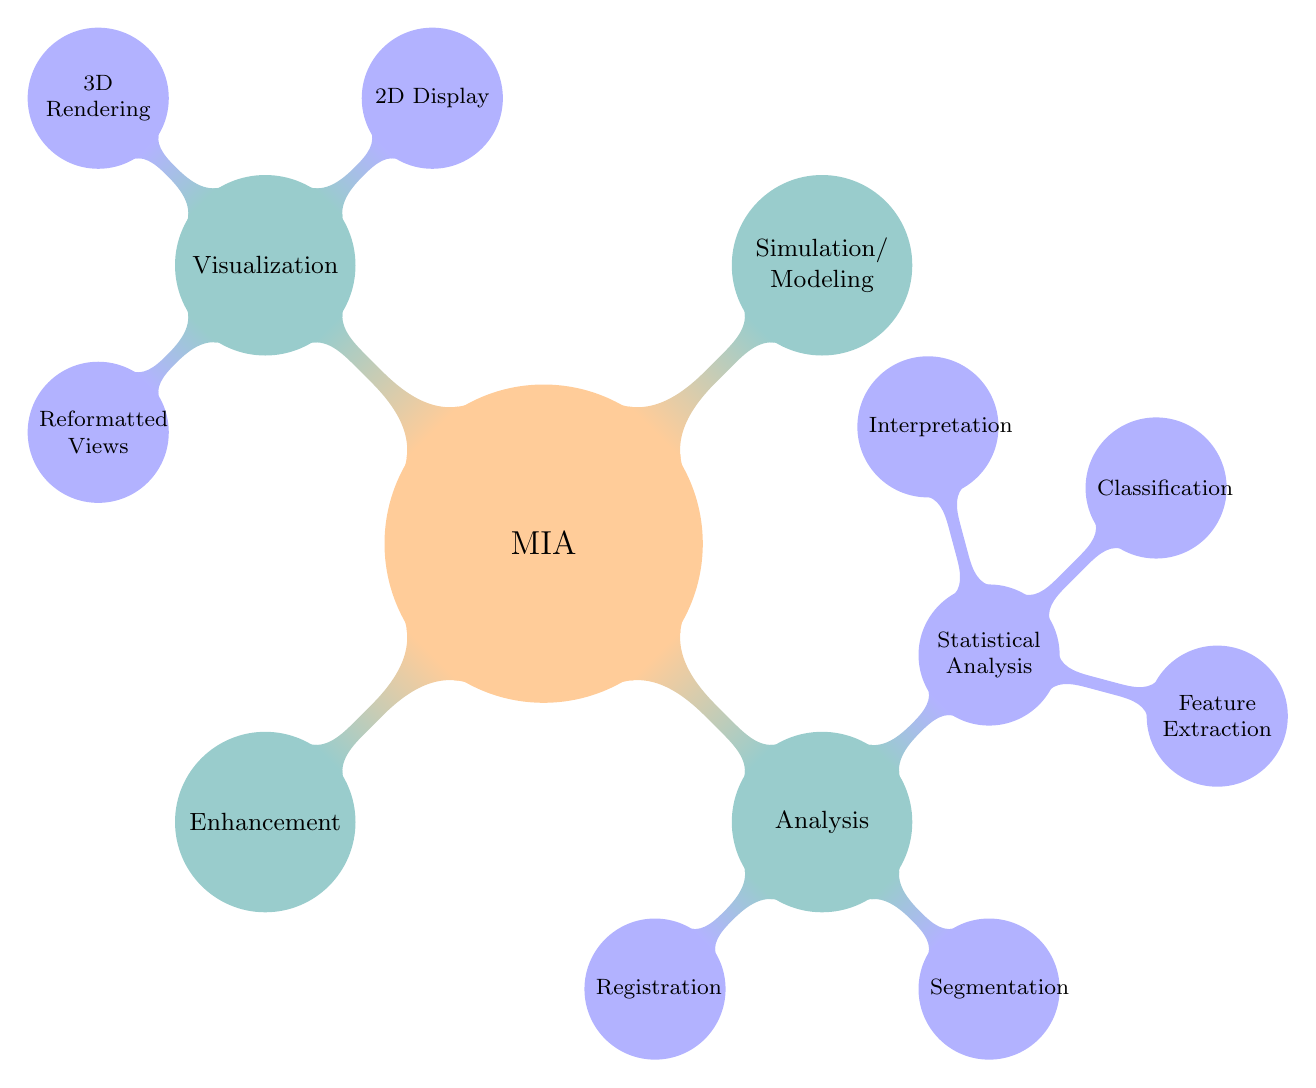
\begin{tikzpicture}[mindmap, grow cyclic, every node/.style=concept, concept
color=orange!40,
	level 1/.append style={level distance=5cm,sibling angle=90},
	level 2/.append style={level distance=3cm,sibling angle=90},
	level 3/.style={level distance=3cm,sibling angle=60}]
\node{\famname}
	child[concept color=teal!40] { node {Enhancement}}
	child[concept color=teal!40] { node {Analysis}
    	child[concept color=blue!30] { node {Registration}}
	    child[concept color=blue!30,] { node {Segmentation}}
	    child[concept color=blue!30] { node {Statistical Analysis}
	        child { node {Feature Extraction}}
	        child { node {Classification}}
	        child { node {Interpretation}}
	}}
	child[concept color=teal!40] { node {Simulation/\\Modeling}}
    child[concept color=teal!40] { node {Visualization}
	    child[concept color=blue!30] { node {2D Display}}
	    child[concept color=blue!30] { node {3D Rendering}}
	    child[concept color=blue!30] { node {Reformatted Views}}
    	}
;
\end{tikzpicture}
}

\end{frame}

%%%%%%%%%%%%%%%%%%%%%%%%%%%%%%%%%%%%%%%%%%%%%%%%%%%%%%%%%%%%%%%%%%%%%%%%%%%%%

\begin{frame}
\frametitle{Overall Process}

\begin{enumerate}
%\item Identify the domain
\item \emph{Domain Expert}: Create a top ten list
%\item Brief \emph{Domain Expert}
\item Initial list of candidate software packages
\item \emph{Domain Expert}: Vet domain software list
\item Domain Analysis, Software Features
\item \emph{Domain Expert}: Vet domain analysis / features
%\item Gather source code and documentation for software
\item Collect empirical measures (stars, forks, lines of code, etc.)
\item Measure using measurement template
\item Interview developers (pain points)
\item Use AHP process to rank the software packages
\item \emph{Domain Expert}: Vet AHP ranking
\item \emph{Domain Expert}: Review recommendations %$\Leftarrow$
\end{enumerate}

\end{frame}

%%%%%%%%%%%%%%%%%%%%%%%%%%%%%%%%%%%%%%%%%%%%%%%%%%%%%%%%%%%%%%%%%%%%%%%%%%%%%

\begin{frame}
\frametitle{Vet Software List}

\bi
\item \structure{How does our list compare to the domain expert's list?}
\item \structure{Is any software missing?}
\item \structure{Is there software that should be included?}
\item \structure{Any other questions/comments or concerns?}
\ei
  
\end{frame}

%%%%%%%%%%%%%%%%%%%%%%%%%%%%%%%%%%%%%%%%%%%%%%%%%%%%%%%%%%%%%%%%%%%%%%%%%%%%%

\begin{frame}[plain]
%\frametitle{SOP Software List}

\begin{multicols}{2}	
	\bi
      \item 3D Slicer
      \item  Ginkgo CADx
      \item XMedCon
      \item Weasis
      \item MRIcroGL
      \item SMILI
      \item ImageJ
      \item Fiji
      \item DicomBrowser
        \item 3DimViewer
        \item Horos
        \item OsiriX Lite
        \item dwv
        \item Drishti
        \item BioImage Suite Web
        \item OHIF Viewer
          \item Slice:Drop
          \item GATE
          \item ITK-SNAP
          \item ParaView
          \item MatrixUser
          \item DICOM Viewer
          \item INVESALIUS 3
            \item medInria
            \item dicompyler
            \item MicroView
            \item Papaya
            \item AMIDE
            \item Gwyddion \ei
\end{multicols}

\end{frame}

%%%%%%%%%%%%%%%%%%%%%%%%%%%%%%%%%%%%%%%%%%%%%%%%%%%%%%%%%%%%%%%%%%%%%%%%%%%%%

\begin{frame}
\frametitle{Common With Domain Expert List}

\bi
\item 3DSlicer
\item Horos
\item ImageJ
\item Fiji (a ``batteries-included" distribution of ImageJ)
\item Mango (on the initial list, but not the final list)
\item Papaya (the web version of Mango)
\item MRIcroGL (MRIcron development has moved to MRIcroGL)
\ei

\end{frame}

%%%%%%%%%%%%%%%%%%%%%%%%%%%%%%%%%%%%%%%%%%%%%%%%%%%%%%%%%%%%%%%%%%%%%%%%%%%%%

\begin{frame}
\frametitle{Only on Domain Expert List}

\bi
\item AFNI \hyperlink{https://afni.nimh.nih.gov}{https://afni.nimh.nih.gov}
\item FSL \hyperlink{https://fsl.fmrib.ox.ac.uk/fsl/fslwiki}{https://fsl.fmrib.ox.ac.uk/fsl/fslwiki} 
\item Freesurfer \hyperlink{https://surfer.nmr.mgh.harvard.edu}{https://surfer.nmr.mgh.harvard.edu} 
\item Tarquin \hyperlink{http://tarquin.sourceforge.net}{http://tarquin.sourceforge.net}  (for MRSpectroscopy data)
\item Diffusion Toolkit  \hyperlink{http://trackvis.org/dtk/}{http://trackvis.org/dtk/} (diffusion toolkit and trakVis)
\item MRItrix \hyperlink{https://www.mrtrix.org}{https://www.mrtrix.org}
\ei

\end{frame}

%%%%%%%%%%%%%%%%%%%%%%%%%%%%%%%%%%%%%%%%%%%%%%%%%%%%%%%%%%%%%%%%%%%%%%%%%%%%%

\begin{frame}
\frametitle{Only on SOP List}

\begin{multicols}{2}	
\bi
\item Ginkgo CADx
\item XMedCon
\item Weasis
\item SMILI
\item DicomBrowser
\item 3DimViewer
\item OsiriX Lite
\item dwv
\item Drishti
\item BioImage Suite Web
\item OHIF Viewer
\item Slice:Drop
\item GATE
\item ITK-SNAP
\item ParaView
\item MatrixUser
\item DICOM Viewer
\item INVESALIUS 3
\item medInria
\item dicompyler
\item MicroView
\item AMIDE
\item Gwyddion
\ei
\end{multicols}

\end{frame}

%%%%%%%%%%%%%%%%%%%%%%%%%%%%%%%%%%%%%%%%%%%%%%%%%%%%%%%%%%%%%%%%%%%%%%%%%%%%%

\begin{frame}
\frametitle{Domain Analysis and Features}

\bi
\item \structure{Can we work together on doing the following for the
    paper?}
  \bi
\item Domain analysis
\item List of features
\item Matrix of software related to features \ei \ei

\end{frame}

%%%%%%%%%%%%%%%%%%%%%%%%%%%%%%%%%%%%%%%%%%%%%%%%%%%%%%%%%%%%%%%%%%%%%%%%%%%%%

\begin{frame}
\frametitle{Measurements Made}

\be
\item Installability
\item Correctness and verifiability
\item Surface reliability
\item Surface robustness
\item Surface usability
\item Maintainability
\item Reusability
\item Surface understandability
\item Visibility and transparency
 \ee
  
\end{frame}

%%%%%%%%%%%%%%%%%%%%%%%%%%%%%%%%%%%%%%%%%%%%%%%%%%%%%%%%%%%%%%%%%%%%%%%%%%%%%

\begin{frame}
\frametitle{Maintainability Measurement}

\bigskip

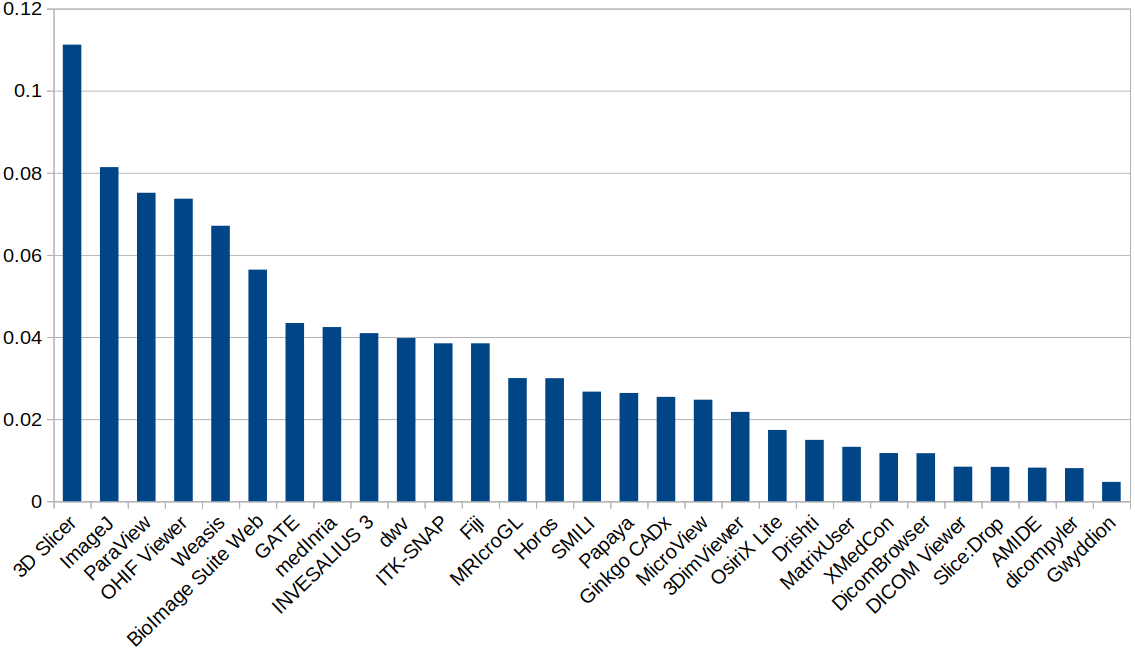
\includegraphics[width=1.0\textwidth]{maintainability_scores.png}

    \structure{Does anything stand out?}

\end{frame}

%%%%%%%%%%%%%%%%%%%%%%%%%%%%%%%%%%%%%%%%%%%%%%%%%%%%%%%%%%%%%%%%%%%%%%%%%%%%%

\begin{frame}
\frametitle{Domain Expert: Ranking Follow-Up}

\bi
\item \structure{Can you review the full ranking measurements?}
\bi
\item There are 9 measurements
\item The write up is about 10 pages long \ei \ei

\end{frame}

%%%%%%%%%%%%%%%%%%%%%%%%%%%%%%%%%%%%%%%%%%%%%%%%%%%%%%%%%%%%%%%%%%%%%%%%%%%%%

\begin{frame}
\frametitle{Pain Points from Developer Interviews}

\structure{Do these fit with your experience?}
\bi
\item Lack of time to 1) implement all requested new features 2) write and maintain good documents 3) review all contributions from the community
\item It is difficult to find or keep the members with experience in both software development and medical imaging
\item Lack of funding for software development (especially for maintenance)
\item No organizations to help with developing high quality software
\item Difficulty to get test data
\item Difficulty to achieve cross-platform compatibility: 1) native app - more time and work 2) web app w/o server - worse performance 3) web app w/ servers - more cost
\ei

\end{frame}

%%%%%%%%%%%%%%%%%%%%%%%%%%%%%%%%%%%%%%%%%%%%%%%%%%%%%%%%%%%%%%%%%%%%%%%%%%%%%

\begin{frame}
\frametitle{Recommendations}

\structure{Do these seem feasible?  What other ideas do we have?}
\bi
\item Consult with software development organization
  \bi
\item Better Scientific Software (BSSw)
\item Software Sustainability Institute
\item Software Carpentry
  \ei
\item Citations for software (Katz project)
  \item Redefine productivity to include time working on tasks like testing, continuous
    integration and documentation
\ei

\end{frame}

%%%%%%%%%%%%%%%%%%%%%%%%%%%%%%%%%%%%%%%%%%%%%%%%%%%%%%%%%%%%%%%%%%%%%%%%%%%%%

\begin{frame}
\frametitle{Publication}

\bi
\item \structure{Who do you see as the targeted readers?}
\item \structure{Where should we publish this paper?}
\ei

\end{frame}

%%%%%%%%%%%%%%%%%%%%%%%%%%%%%%%%%%%%%%%%%%%%%%%%%%%%%%%%%%%%%%%%%%%%%%%%%%%%%

\begin{frame}
\frametitle{Developer Questions}

\bi
\item \structure{What experience do you, or your students, have with developing
    software?}
\item \structure{How big would the development group be?}
\item \structure{What is the typical background of a developer?}
\item \structure{How many users would you software typically have?}
\item \structure{What is the typical background of a user?}
\item \structure{Currently, what are the most significant obstacles in your
    development process?}
\item \structure{How might you change your development process to remove or
    reduce these obstacles?}
\item \structure{How does documentation fit into your development process? Would improved
  documentation help with the obstacles you typically face?}      
\ei

\end{frame}

%%%%%%%%%%%%%%%%%%%%%%%%%%%%%%%%%%%%%%%%%%%%%%%%%%%%%%%%%%%%%%%%%%%%%%%%%%%%%

\begin{frame}
\frametitle{Developer Questions Continued}

\bi
\item \structure{In the past, is there any major obstacle to your development process that
  has been solved? How did you solve it?}
\item \structure{What is your software development model? For example, waterfall, agile,
  etc.}
\item \structure{What is your project management process? Do you think improving this
  process can tackle the current problem? Were any project management tools
  used?}
\item \structure{Was it hard to ensure the correctness of the software? If there
    were any obstacles, what methods have been considered or practiced to
    improve the situation? If practiced, did it work?}
\ei

\end{frame}

%%%%%%%%%%%%%%%%%%%%%%%%%%%%%%%%%%%%%%%%%%%%%%%%%%%%%%%%%%%%%%%%%%%%%%%%%%%%%

\begin{frame}
\frametitle{Developer Questions Continued}

\bi
\item \structure{When designing the software, did you consider the ease of
    future changes? For example, will it be hard to change the structure of
    the system, modules or code blocks? What measures have been taken to ensure
    the ease of future changes and maintainance?}
\item \structure{Provide instances where users have misunderstood the
    software. What, if any, actions were taken to address understandability
    issues?}
\item \structure{What, if any, actions were taken to address usability issues?}
\item \structure{Do you think the current documentation can clearly convey all
    necessary knowledge to the users? If yes, how did you successfully achieve
    it? If no, what improvements are needed?}
\ei

\end{frame}

%%%%%%%%%%%%%%%%%%%%%%%%%%%%%%%%%%%%%%%%%%%%%%%%%%%%%%%%%%%%%%%%%%%%%%%%%%%%%

\begin{frame}
\frametitle{Developer Questions Continued}

\bi
\item \structure{Do you have any concern that your computational results won't
    be reproducible in the future? Have you taken any steps to ensure
    reproducibility?}  \ei

\end{frame}

%%%%%%%%%%%%%%%%%%%%%%%%%%%%%%%%%%%%%%%%%%%%%%%%%%%%%%%%%%%%%%%%%%%%%%%%%%%%%

\end{document}
